\documentclass{telkomnika}

%%required package. add for your convenient, but do not remove the initial
\setlength{\headsep}{0.15in}
\usepackage{amsmath, amsfonts, amssymb, float, fancyhdr}
\usepackage[figuresright]{rotating}
\usepackage{authblk, graphicx, indentfirst, lastpage, lipsum}
\usepackage{pifont}
\renewcommand{\Authsep}{, }
\renewcommand{\Authand}{, }
\renewcommand{\Authands}{, }
\setlength{\affilsep}{0cm}
\renewcommand\Authfont{\normalsize}
\renewcommand\Affilfont{\fontsize{8}{10}\mdseries}
\makeatletter
\renewcommand{\@biblabel}[1]{[#1]\hfill}
\renewcommand\AB@authnote[1]{\textsuperscript{\normalfont\bfseries#1}}
\makeatother
\usepackage[font=normalsize]{subfig, caption}
\usepackage{epstopdf}
\usepackage[left=3cm, right=2.5cm, top=2.5cm, bottom=2.5cm, includehead, includefoot]{geometry}
\usepackage[justification=centering]{caption}
\captionsetup{labelsep=period}
\usepackage{titlesec}
\usepackage{xcolor}
\titleformat{\section}
{\normalfont\normalsize\bfseries\uppercase}{\thesection}{1.7em}{}
\titleformat{\subsection}
{\normalfont\normalsize\bfseries}{\thesubsection}{.95em}{}
\titleformat{\subsubsection}
{\bfseries}{\thesubsubsection}{.2em}{}
\titlespacing*{\section}{0cm}{0.7cm}{0cm}
\usepackage{enumitem}
\usepackage[numbers,sort&compress]{natbib}
\usepackage{ragged2e}
\usepackage{hyperref,graphicx}
\usepackage{multirow}


%%leave copyright info to the editor
\CopyrightLine[]{}{\textit{This is an open access article under the \textcolor{blue}{\underline{CC BY-SA}} license.}
\vspace{.5em}}

%%author
\author[1,2]{\bfseries Saad Mekhilef}
\author[3]{\bfseries Oscar Castillo}
\author[3]{\bfseries Patricia Melin}

%%author's affiliation
\affil[1]{Power Electronics and Renewable Energy Research Laboratory (PEAR-L), University of Malaya, Kuala Lumpur, Malaysia (8 pt)}
\affil[2]{Department of Electrical Engineering, Faculty of Engineering, University of Malaya, Kuala Lumpur, Malaysia}
\affil[3]{Division of Graduate Studies, Tijuana Institute of Technology, Tijuana, Mexico}

%%title and shortitle (for footer)
\title{Mean End Analysis Decision Making Model in Santorini Board Game}
\shorttitle{Paper’s title should be the fewest possible words that accurately describe ... (First Author)}

%%starting
\begin{document}
\setcounter{page}{1}

%%indentation. do not change
\setlength{\parindent}{1.27cm}

%%header and footer setting. do not change
\pagestyle{fancy}
\fancyhfoffset{0cm}

%%journal info
\journalname{TELKOMNIKA Telecommunication, Computing, Electronics and Control}
\journalshortname{TELKOMNIKA Telecommun Comput El Control}
\journalhomepage{http://journal.uad.ac.id/index.php/TELKOMNIKA}
\vol{99}
\no{1}
\months{February}
\years{2099}
\issn{1693-6930}
\DOI{10.12928}
\pagefirst{1}
\pagelast{1x}
\IDpaper{paperID}


%%build title
\maketitle


%%border setting. do not change
\hrule
\vspace{.1em}
\hrule
\vspace{.5em}
\noindent
\parbox[t][][s]{0.315\textwidth}{%
\textbf{Article Info}
\vspace{.5em}
\hrule
\vspace{.5em}
\begin{history}
\vspace{.5em}

%%article info. editor's privilege
Received mm dd, yyyy

Revised mm dd, yyyy

Accepted mm dd, yyyy

\vspace{.7em}
\end{history}
\vspace{.5em}
\hrule
\vspace{.5em}
\begin{keyword} 
\vspace{.5em}
%%write keyword here. separate by \sep
First keyword \sep Second keyword \sep Third keyword \sep Fourth keyword \sep Fifth keyword
\vspace{.5em}
\end{keyword}
\vspace{\fill}
}
\parbox{0.020\textwidth}{\hspace{.5em}}
\parbox[t][][s]{0.65\textwidth}{%
\begin{abstract}
\vspace{.3em}
%% Text of abstract
An abstract is often presented separate from the article, so it must be able to stand alone. A well-prepared abstract enables the reader to identify the basic content of a document quickly and accurately, to determine its relevance to their interests, and thus to decide whether to read the document in its entirety. The abstract should be informative and completely self-explanatory, provide a clear statement of the problem, the proposed approach or solution, and point out major findings and conclusions. \textbf{The Abstract should be 100 to 200 words in length}. References should be avoided, but if essential, then cite the author(s) and year(s). Standard nomenclature should be used, and non-standard or uncommon abbreviations should be avoided, but if essential they must be defined at their first mention in the abstract itself. No literature should be cited. The keyword list provides the opportunity to add 5 to 7 keywords, used by the indexing and abstracting services, in addition to those already present in the title (9 pt).
\end{abstract}
}
\parbox[l]{\textwidth}{%
\rule{0.275\textwidth}{0.5pt} \hspace{0.5cm} \hrulefill
\\
\emph{\textbf{Corresponding Author:}}
\vspace{.5em}\\
%% correspondence info. separate by \\
Saad Mekhilef\\
Power Electronics and Renewable Energy Research Laboratory (PEAR-L), University of Malaya\\
Balai Cerap UTM, Lengkok Suria, 81310 Skudai, Johor, Malaysia\\
Email: saad@um.edu.my
}
\vspace{.5em}
\hrule
\vspace{.1em}
\hrule


%% main text

\section{Introduction}
\label{}
The main text format consists of a flat left-right columns on A4 paper (quarto). The margin text from the left and top are 2.5 cm, right and bottom are 2 cm. The manuscript is written in Microsoft Word, single space, Time New Roman 10 pt, and maximum 12 pages for original research article, or maximum 16 pages for review/survey paper, which can be downloaded at the website: http://journal.uad.ac.id/index.php/TELKOMNIKA.

A title of article should be the fewest possible words that accurately describe the content of the paper. The title should be succinct and informative and no more than about 12 words in length. Do not use acronyms or abbreviations in your title and do not mention the method you used, unless your paper reports on the development of a new method. Titles are often used in information-retrieval systems. Avoid writing long formulas with  subscripts in the title.. Omit all waste words such as \textit{"A study of ...", "Investigations of ...", "Implementation of ...”, "Observations on ...", "Effect of.....", “Analysis of …”}, “Design of…” etc. 

A concise and factual abstract is required. The abstract should state briefly the purpose of the research, the principal results and major conclusions. An abstract is often presented separately from the article, so it must be able to stand alone. For this reason, References should be avoided, but if essential, then cite the author(s) and year(s). Also, non-standard or uncommon abbreviations should be avoided, but if essential they must be defined at their first mention in the abstract itself. Immediately after the abstract, provide a maximum of 7 keywords, using American spelling and avoiding general and plural terms and multiple concepts (avoid, for example, 'and', 'of'). Be sparing with abbreviations: only abbreviations firmly established in the field may be eligible. These keywords will be used for indexing purposes. Indexing and abstracting services depend on the accuracy of the title, extracting from it keywords useful in cross-referencing and computer searching. An improperly titled paper may never reach the audience for which it was intended, so be specific. 

The Introduction section should provide: i) a clear background, ii) a clear statement of the problem, iii) the relevant literature on the subject, iv) the proposed approach or solution, and v) the new value of research which it is innovation (within 3-6 paragraphs). It should be understandable to colleagues from a broad range of scientific disciplines. Organization and citation of the bibliography are made in Institute of Electrical and Electronics Engineers (IEEE) style in sign [1], [2] and so on. The terms in foreign languages are written italic (italic). The text should be divided into sections, each with a separate heading and numbered consecutively [3]. The section or subsection headings should be typed on a separate line, e.g., 1. INTRODUCTION. A full article usually follows a standard structure: \textbf{1. Introduction, 2. The Comprehensive Theoretical Basis and/or the Proposed Method/Algorithm} \textit{(optional)},\textbf{ 3. Method, 4. Results and Discussion, and 5. Conclusion.} The structure is well-known as \textbf{IMRaD} style.

Literature review that has been done author used in the section "INTRODUCTION" to explain 
the difference of the manuscript with other papers, that it is innovative, it are used in the section "METHOD" to describe the step of research and used in the section "RESULTS AND DISCUSSION" to support the analysis of the results [2]. If the manuscript was written really have high originality, which proposed a new method or algorithm, the additional section after the "INTRODUCTION" section and before the "METHOD" section can be added to explain briefly the theory and/or the proposed method/algorithm [4].


\section{Method}
\label{}
Explaining research chronological, including research design, research procedure (in the form of algorithms, Pseudocode or other), how to test and data acquisition [5]–[7]. The description of the course of research should be supported references, so the explanation can be accepted scientifically [2], [4]. Figures 1-2 and Table 1 are presented center, as shown below and cited in the manuscript [5], [8]–[13]. The nodes energy consumption in network OHCRP (50\%\ DSr) vs SPEED has been illustrated in Figure 2(a) and network OHCRP (50% DSr) vs THVR has been illustrated Figure 2(b).


\begin{table}[H]
\centering
\fontsize{8pt}{10pt}\selectfont
\caption{The performance of ...}
\begin{tabular}{lcr}
\hline
Variable & Speed (rpm) & Power (kW) \\
\hline
x & 10 & 8.6 \\
y & 15 & 12.4 \\
z & 20 & 15.3 \\
\hline
\end{tabular}
\end{table}

\begin{figure}[H]
\centering
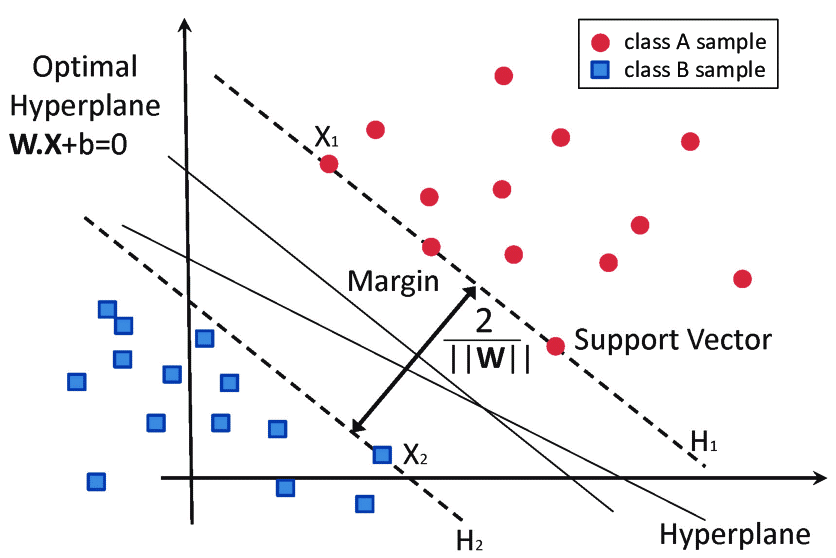
\includegraphics[scale=0.4]{figure1}
%% make sure to add \vspace{.7em} before figure's caption
\vspace{.7em}
\caption{Effects of selecting different switching under dynamic condition}
\end{figure}

\begin{figure}[H]
\centering
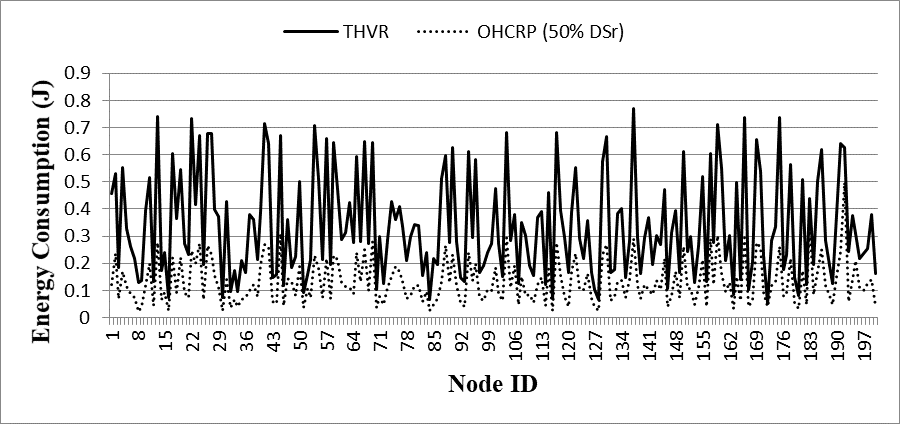
\includegraphics[scale=0.7]{figure2(a)}\\
(a)\\
\vspace{.7em}
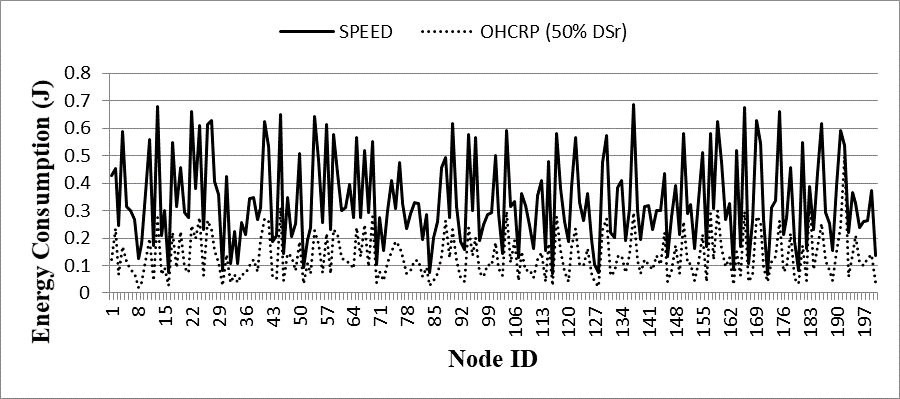
\includegraphics[scale=0.7]{figure2(b)}\\
(b)\\
	%% make sure to add \vspace{.7em} before figure's caption
\vspace{.7em}
\caption{Nodes energy consumption in network (a) OHCRP (50\%\ DSr) vs SPEED and \linebreak (b) OHCRP (50\%\ DSr) vs THVR}
\end{figure}


\section{Result and Discussion}
\label{}
In this section, it is explained the results of research and at the same time is given 
the comprehensive discussion. Results can be presented in figures, graphs, tables and others that make 
the reader understand easily [14], [15]. The discussion can be made in several sub-sections.


\subsection{Sub section 1}
Equations should be placed at the center of the line and provided consecutively with equation numbers in parentheses flushed to the right margin, as in (1). The use of Microsoft Equation Editor or MathType is preferred.


\begin{equation}
E_v - E = \frac{\hbar}{2.m}(k_x^2 + k_y^2)
\end{equation}
%% make sure to add \vspace{.005em} after the end of equation
\vspace{.005em}
\\All symbols that have not been mentioned in the equation should be explained in the following text.

\subsection{Sub section 2}
Proper citation of other works should be made to avoid plagiarism. When referring to a reference item, please use the reference number as in [16] or [17] for multiple references. The use of ”Ref [18]...” should be employed for any reference citation at the beginning of sentence. For any reference with more than 3 or more authors, only the first author is to be written followed by et al. (e.g. in [19]). Examples of reference items of different categories shown in the References section. Each item in the references section should be typed using 8 pt font size [20]–[25].

\subsubsection {Subsub section 1}
yy

\subsubsection {Subsub section 2}
zz

\section{Conclusion}
\label{}
Provide a statement that what is expected, as stated in the "INTRODUCTION" section can ultimately result in "RESULTS AND DISCUSSION" section, so there is compatibility. Moreover, it can also be added the prospect of the development of research results and application prospects of further studies into the next (based on results and discussion).

\section*{Acknowledgement}
\label{}
The acknowledgment section is optional. The funding source of the research can be put here.

\section*{REFERENCES}
\label{}
\footnotesize
The main references are international journals and proceedings. All references should be to the most pertinent, up-to-date sources \textbf{and the minimum of references} are \textbf{25 entries} (for original research paper) and \textbf{50 entries} (for review/survey paper). References are written in \textbf{IEEE style}. For more complete guide can be accessed at (http://ipmuonline.com/guide/refstyle.pdf). Use of a tool such as \textbf{EndNote, Mendeley}, or \textbf{Zotero} for reference management and formatting, and choose \textbf{IEEE style}. Please use a consistent format for references-see examples (8 pt):

\subsection*{[1] Journal/Periodicals}
\footnotesize
\begin{flushleft}
\textsl{Basic Format:\\}
\end{flushleft}
\vspace{-1.1em} 
J. K. Author, “Title of paper,” \textsl{Abbrev. Title of Journal/Periodical}, vol. x, no. x, pp. xx-xx, Abbrev. Month, year, doi: xxx.\\ 
\emph{Examples:}
\begin{enumerate} [leftmargin=*, topsep=0.3ex, itemsep=0.3ex, parsep=0.2ex]
\footnotesize
\item[$-$] M. M. Chiampi and L. L. Zilberti, “Induction of electric field in human bodies moving near MRI: An efficient BEM computational procedure,” \textsl{IEEE Transaction on Biomedical Engineering}, vol. 58, pp. 2787–2793, Oct. 2011, doi: 10.1109/TBME.2011.2158315.
\item[$-$] R. Fardel, M. Nagel, F. Nuesch, T. Lippert, and A. Wokaun, “Fabrication of organic light emitting diode pixels by laser-assisted forward transfer,” \textsl{Appl. Phys. Lett.}, vol. 91, no. 6, Aug. 2007, Art. no. 061103, doi: 10.1063/1.2759475.
\end{enumerate}


\subsection*{[2]	Conference Proceedings}
\footnotesize
\begin{flushleft}
\textsl{Basic Format:\\}
\end{flushleft}
\vspace{-1.1em} 
J. K. Author, “Title of paper,” \textsl{in Abbreviated Name of Conf.}, (location of conference is optional), year, pp. xxx–xxx, doi: xxx. \\
\emph{Examples:}
\begin{enumerate} [leftmargin=*, topsep=0.3ex, itemsep=0.3ex, parsep=0.2ex]
\footnotesize
\item[$-$] G. Veruggio, “The EURON roboethics roadmap,” in \textsl{Proc. Humanoids ’06: 6th IEEE-RAS Int. Conf. Humanoid Robots}, 2006, pp. 612–617, doi: 10.1109/ICHR.2006.321337. 
\item[$-$]	J. Zhao, G. Sun, G. H. Loh, and Y. Xie, “Energy-efficient GPU design with reconfigurable in-package graphics memory,” in \textsl{Proc. ACM/IEEE Int. Symp. Low Power Electron. Design (ISLPED)}, Jul. 2012, pp. 403–408, doi: 10.1145/2333660.2333752.
\end{enumerate}


\subsection*{[3] Book}
\footnotesize
\begin{flushleft}
\textsl{Basic Format:\\}
\end{flushleft}
\vspace{-1.1em} 
\footnotesize
J. K. Author, “Title of chapter in the book,” in \textsl{Title of His Published Book}, X. Editor, Ed., xth ed. City of Publisher, State (only U.S.), Country: Abbrev. of Publisher, year, ch. x, sec. x, pp. xxx–xxx. \\
\textsl{Examples:}
\begin{enumerate} [leftmargin=*, topsep=0.3ex, itemsep=0.3ex, parsep=0.2ex]
\footnotesize
    \item[$-$] A. Taflove, \textsl{Computational Electrodynamics: The Finite-Difference Time-Domain Method} in Computational Electrodynamics II, vol. 3, 2nd ed. Norwood, MA, USA: Artech House, 1996. 
		\item[$-$] R. L. Myer, “Parametric oscillators and nonlinear materials,” in \textsl{Nonlinear Optics}, vol. 4, P. G. Harper and B. S. Wherret, Eds., San Francisco, CA, USA: Academic, 1977, pp. 47–160.
\end{enumerate}


%% References
%%
%% Following citation commands can be used in the body text:
%% Usage of \cite is as follows:
%%   \cite{key}         ==>>  [#]
%%   \cite[chap. 2]{key} ==>> [#, chap. 2]
%%

%% References with BibTeX database:

\bibliographystyle{IEEEtran}
%\bibliography{<your-bib-database>}
%% Authors are advised to use a BibTeX database file for their reference list.
%% The provided style IEEEtran.bst formats references is generally used.

%% For references without a BibTeX database:

\begin{thebibliography} {99} 
\footnotesize
\itemsep 0pt 


%%The main references are international journals and proceedings. All references should be to the most pertinent, up-to-date sources and the minimum of references are 25. References are written in IEEE style. Please use a consistent format for references – see examples below:

%% \bibitem must have the following form:
%%   \bibitem{key}...
%%

 \bibitem{1} M. Sigala, A. Beer, L. Hodgson, and A. O’Connor, \emph{Big Data for Measuring the Impact of Tourism Economic Development Programmes: A Process and Quality Criteria Framework for Using Big Data}. 2019.

\bibitem{2} G. Nguyen et al., “Machine Learning and Deep Learning frameworks and libraries for large-scale data mining: a survey,” \textsl{Artif. Intell. Rev.}, vol. 52, no. 1, pp. 77–124, 2019, doi: 10.1007/s10462-018-09679-z

\bibitem{3} C. Shorten and T. M. Khoshgoftaar, “A survey on Image Data Augmentation for Deep Learning,” \textsl{J. Big Data}, vol. 6, no. 1, 2019, doi: 10.1186/s40537-019-0197-0.

\bibitem{4} R. Vinayakumar, M. Alazab, K. P. Soman, P. Poornachandran, A. Al-Nemrat, and S. Venkatraman, “Deep Learning Approach for Intelligent Intrusion Detection System,” \textsl{IEEE Access}, vol. 7, pp. 41525–41550, 2019, doi: 10.1109/ACCESS.2019.2895334.

\bibitem{5} K. Sivaraman, R. M. V. Krishnan, B. Sundarraj, and S. Sri Gowthem, “Network failure detection and diagnosis by analyzing syslog and SNS data: Applying big data analysis to network operations,” \textsl{Int. J. Innov. Technol. Explor. Eng.}, vol. 8, no. 9 Special Issue 3, pp. 883–887, 2019, doi: 10.35940/ijitee.I3187.0789S319.

\bibitem{6} A. D. Dwivedi, G. Srivastava, S. Dhar, and R. Singh, “A decentralized privacy-preserving healthcare blockchain for IoT,” \textsl{Sensors (Switzerland)}, vol. 19, no. 2, pp. 1–17, 2019, doi: 10.3390/s19020326.

\bibitem{7} F. Al-Turjman, H. Zahmatkesh, and L. Mostarda, “Quantifying uncertainty in internet of medical things and big-data services using intelligence and deep learning,” \textsl{IEEE Access}, vol. 7, pp. 115749–115759, 2019, doi: 10.1109/ACCESS.2019.2931637.

\bibitem{8} S. Kumar and M. Singh, “Big data analytics for healthcare industry: Impact, applications, and tools,” \textsl{Big Data Min. Anal.}, vol. 2, no. 1, pp. 48–57, 2019, doi: 10.26599/BDMA.2018.9020031

\bibitem{9} L. M. Ang, K. P. Seng, G. K. Ijemaru, and A. M. Zungeru, “Deployment of IoV for Smart Cities: Applications, Architecture, and Challenges,” \textsl{IEEE Access}, vol. 7, pp. 6473–6492, 2019, doi: 10.1109/ACCESS.2018.2887076.

\bibitem{10} B. P. L. Lau et al., “A survey of data fusion in smart city applications,” \textsl{Inf. Fusion}, vol. 52, no. January, pp. 357–374, 2019, doi: 10.1016/j.inffus.2019.05.004.

\bibitem{11} Y. Wu et al., “Large scale incremental learning,” \textsl{Proc. IEEE Comput. Soc. Conf. Comput. Vis. Pattern Recognit.}, vol. 2019-June, pp. 374–382, 2019, doi: 10.1109/CVPR.2019.00046.

\bibitem{12} A. Mosavi, S. Shamshirband, E. Salwana, K. wing Chau, and J. H. M. Tah, “Prediction of multi-inputs bubble column reactor using a novel hybrid model of computational fluid dynamics and machine learning,” \textsl{Eng. Appl. Comput. Fluid Mech.}, vol. 13, no. 1, pp. 482–492, 2019, doi: 10.1080/19942060.2019.1613448.

\bibitem{13} V. Palanisamy and R. Thirunavukarasu, “Implications of big data analytics in developing healthcare frameworks – A review,” \textsl{J. King Saud Univ. - Comput. Inf. Sci.}, vol. 31, no. 4, pp. 415–425, 2019, doi: 10.1016/j.jksuci.2017.12.007.

\bibitem{14} J. Sadowski, “When data is capital: Datafication, accumulation, and extraction,” \textsl{Big Data Soc.}, vol. 6, no. 1, pp. 1–12, 2019, doi: 10.1177/2053951718820549.

\bibitem{15} J. R. Saura, B. R. Herraez, and A. Reyes-Menendez, “Comparing a traditional approach for financial brand communication analysis with a big data analytics technique,” \textsl{IEEE Access}, vol. 7, pp. 37100–37108, 2019, doi: 10.1109/ACCESS.2019.2905301.

\bibitem{16} D. Nallaperuma et al., “Online Incremental Machine Learning Platform for Big Data-Driven Smart Traffic Management,” textsl{IEEE Trans. Intell. Transp. Syst.}, vol. 20, no. 12, pp. 4679–4690, 2019, doi: 10.1109/TITS.2019.2924883.

\bibitem{17} S. Schulz, M. Becker, M. R. Groseclose, S. Schadt, and C. Hopf, “Advanced MALDI mass spectrometry imaging in pharmaceutical research and drug development,” \textsl{Curr. Opin. Biotechnol.}, vol. 55, pp. 51–59, 2019, doi: 10.1016/j.copbio.2018.08.003.

\bibitem{18} C. Shang and F. You, “Data Analytics and Machine Learning for Smart Process Manufacturing: Recent Advances and Perspectives in the Big Data Era,” \textsl{Engineering}, vol. 5, no. 6, pp. 1010–1016, 2019, doi: 10.1016/j.eng.2019.01.019.

\bibitem{19} Y. Yu, M. Li, L. Liu, Y. Li, and J. Wang, “Clinical big data and deep learning: Applications, challenges, and future outlooks,” \textsl{Big Data Min. Anal.}, vol. 2, no. 4, pp. 288–305, 2019, doi: 10.26599/BDMA.2019.9020007.

\bibitem{20} M. Huang, W. Liu, T. Wang, H. Song, X. Li, and A. Liu, “A queuing delay utilization scheme for on-path service aggregation in services-oriented computing networks,” \textsl{IEEE Access}, vol. 7, pp. 23816–23833, 2019, doi: 10.1109/ACCESS.2019.2899402.

\bibitem{21} G. Xu, Y. Shi, X. Sun, and W. Shen, “Internet of things in marine environment monitoring: A review,” \textsl{Sensors (Switzerland)}, vol. 19, no. 7, pp. 1–21, 2019, doi: 10.3390/s19071711.

\bibitem{22} M. Aqib, R. Mehmood, A. Alzahrani, I. Katib, A. Albeshri, and S. M. Altowaijri, \textsl{Smarter traffic prediction using big data, in-memory computing, deep learning and gpus}, vol. 19, no. 9. 2019.

\bibitem{23} S. Leonelli and N. Tempini, D\textsl{ata Journeys in the Sciences}. 2020.

\bibitem{24} N. Stylos and J. Zwiegelaar, \textsl{Big Data as a Game Changer: How Does It Shape Business Intelligence Within a Tourism and Hospitality Industry Context?} 2019.

\bibitem{25} Q. Song, H. Ge, J. Caverlee, and X. Hu, “Tensor completion algorithms in big data analytics,” \textsl{arXiv}, vol. 13, no. 1, 2017.

\end{thebibliography}

\newpage

\section*{BIOGRAPHIES OF AUTHORS} 
\small
\textbf{\\The recommended number of authors is at least 2. One of them as a corresponding author.}
\textit{\\Please attach clear photo (3x4 cm) and vita. Example of biographies of authors (9 pt)}:
\small

%% make sure to add \vspace{-.7em} before \begin{biography}
\vspace{.7em} 
\small
\begin{biography}[{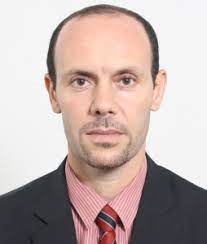
\includegraphics[width=2.5cm,height=4cm,clip,keepaspectratio]{a1}}]
\textbf{Saad Mekhilef} %% Affiliation and educational background.
\href{https://orcid.org/0000-0001-8544-8995}{
\includegraphics[width=0.02\textwidth]{orcid.png}} 
\href{https://scholar.google.co.id/citations?user=0kKMcLYAAAAJ&hl=en}{
\includegraphics[width=0.02\textwidth]{gscholar.png}}
\href{https://www.scopus.com/authid/detail.uri?authorId=6603317449}{
\includegraphics[width=0.02\textwidth]{scopus.png}}
\href{https://publons.com/researcher/1354246/mekhilef-saad/}{
\includegraphics[width=0.02\textwidth]{publons.png}} received the B.Eng. degree in electrical engineering from the University of Setif, Setif, Algeria, in 1995, and the master’s degree in engineering science and the Ph.D. degree in electrical engineering from the University of Malaya, Kuala Lumpur, Malaysia, in 1998 and 2003, respectively. He is currently a Professor and the Director of the Power Electronics and Renewable Energy Research Laboratory, Department of Electrical Engineering, University of Malaya, where he is also the Dean of the Faculty of Engineering. He is also a Distinguished Adjunct Professor with the School of Software and Electrical Engineering, Faculty of Science, Engineering and Technology, Swinburne University of Technology, VIC, Australia. His current research interests include power converter topologies, the control of power converters, renewable energy, and energy efficiency. He can be contacted at email: saad@um.edu.my.
\end{biography}

\begin{biography}[{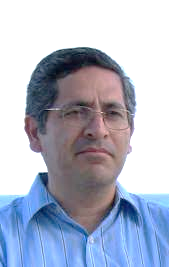
\includegraphics[width=2.5cm,height=4cm,clip,keepaspectratio]{a2}}]
\textbf{Oscar Castillo} %% Affiliation and educational background.
\href{https://orcid.org/0000-0002-7385-5689}{
\includegraphics[width=0.02\textwidth]{orcid.png}} 
\href{https://scholar.google.com/citations?user=1C8gb8IAAAAJ&hl=en}{
\includegraphics[width=0.02\textwidth]{gscholar.png}}
\href{https://www.scopus.com/authid/detail.uri?authorId=7007101709}{
\includegraphics[width=0.02\textwidth]{scopus.png}}
\href{https://publons.com/researcher/1331983/oscar-castillo/}{
\includegraphics[width=0.02\textwidth]{publons.png}} received the D.Sc. degree (Doctor Habilitatus) in computer science from the Polish Academy of Sciences, Warsaw, Poland, with the Dissertation “Soft Computing and Fractal Theory for Intelligent Manufacturing”. He is a Professor of computer science in the Graduate Division, Tijuana Institute of Technology, Tijuana, Mexico. In addition, he is serving as Research Director of computer science and Head of the research group on fuzzy logic and genetic algorithms. He is currently the Vice-President of Hispanic American Fuzzy Systems Association (HAFSA) and President Elect of International Fuzzy Systems Association (IFSA). He has published over 80 journal papers, 6 authored books, 20 edited books, and 200 papers in conference proceedings. His research interests are in Type-2 Fuzzy Logic, Fuzzy Control, Neuro-Fuzzy and Genetic-Fuzzy hybrid approaches. He can be contacted at email: ocastillo@tectijuana.mx.
\end{biography}

\begin{biography}[{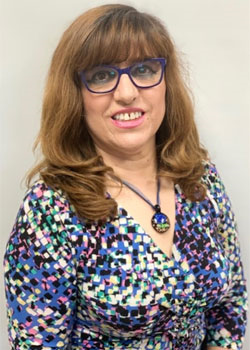
\includegraphics[width=2.5cm,height=4cm,clip,keepaspectratio]{a3}}]
\textbf{Patricia Melin} %% Affiliation and educational background.
\href{https://orcid.org/0000-0001-5798-1426}{
\includegraphics[width=0.02\textwidth]{orcid.png}} 
\href{https://scholar.google.com/citations?user=Ts6JtfMAAAAJ&hl=en}{
\includegraphics[width=0.02\textwidth]{gscholar.png}}
\href{https://www.scopus.com/authid/detail.uri?authorId=7006491873}{
\includegraphics[width=0.02\textwidth]{scopus.png}}
\href{https://publons.com/researcher/1332081/patricia-melin/}{
\includegraphics[width=0.02\textwidth]{publons.png}} received the D.Sc. degree (Doctor Habilitatus D.Sc.) in computer science from the Polish Academy of Sciences, Warsaw, Poland, with the Dissertation “Hybrid Intelligent Systems for Pattern Recognition using Soft Computing”. She is a Professor of Computer Science in the Graduate Division, Tijuana Institute of Technology, Tijuana, Mexico since 1998. In addition, she is serving as Director of Graduate Studies in computer science and Head of the research group on Computational Intelligence (2000–present). Her research interests are in Type-2 Fuzzy Logic, Modular Neural Networks, Pattern Recognition, Neuro-Fuzzy and Genetic-Fuzzy hybrid approaches., She is currently the President of Hispanic American Fuzzy Systems Association (HAFSA) and is the founding Chair of the Mexican Chapter of the IEEE Computational Intelligence Society. She can be contacted at email: pmelin@tectijuana.mx.
\end{biography}


\end{document}

%%
%% End of file `telkomnika.tex'. 